% This file is the Latex source of the Big Data course project
% report. The project contributors are Ali Alavi, Rolf jagerman
% and Ken Tsay.
% The report is written by Ali Alavi, Rolf Jagerman.

%
\documentclass{llncs}
%

\usepackage{graphicx} % for importing images
\usepackage{caption}
\usepackage{subcaption} % for subfigures
\captionsetup{compatibility=false} % to make subfigures compatible with template

\usepackage{url} % for URL references
\usepackage{float} % helps with locating the 
\usepackage[T1]{fontenc}  % providing font encoding
% used for drawing the diagrams
%
\begin{document}
%
\mainmatter              % start of the contributions
\pretolerance=10000  % This avoids long lines
\pagestyle{headings}
%\hyphenation{}

%
\title{Automatic News Generation Based on Twitter}
%
\titlerunning{Automatic News Generation Based on Twitter}  % abbreviated title (for running head)
%                                     also used for the TOC unless
%                                     \toctitle is used
%
\author{Ali Alavi\inst{1} \and Rolf Jagerman\inst{1} \and
Tsay Kai-En\inst{1}}
%
\authorrunning{Ali Alavi, Rolf Jagerman and Tsay Kai-En} % abbreviated author list (for running head)
%
%
\institute{ETH Z\"urich, Z\"urich, Switzerland\\
\email{alavis@ethz.ch, \{rolfj, tsayk\}@student.ethz.ch}
}

\maketitle              % typeset the title of the contribution
%
\section{Introduction}
%
This report presents the current status of the project \textbf{Automatic News Generation Based on Twitter}, 
for \textbf{Big Data} course (code \textit{263-3010-00L}). This project tries to answer the following questions: 
\textit{Can we automatically generate news headlines based on public twitter posts? Can this method of news generation 
perform better than the available news agencies, in terms of speed, reliability and so on?}

We tackle this problem by taking the following steps:

\begin{enumerate}
  \item \textit{Data collection: }Gathering a large set of twitter posts and news headlines 
  \item \textit{Building a classifier: }Use the news headlines to train a classifier
  \item \textit{Labeling the tweets: }Label each tweet using the classifier we previously trained
\end{enumerate}

A big picture of the system is depicted in Figure ~\ref{fig:A big picture of the system}. In the rest of this report we will elaborate on the design and realization of the system.

\begin{figure}[H]
  \centering
  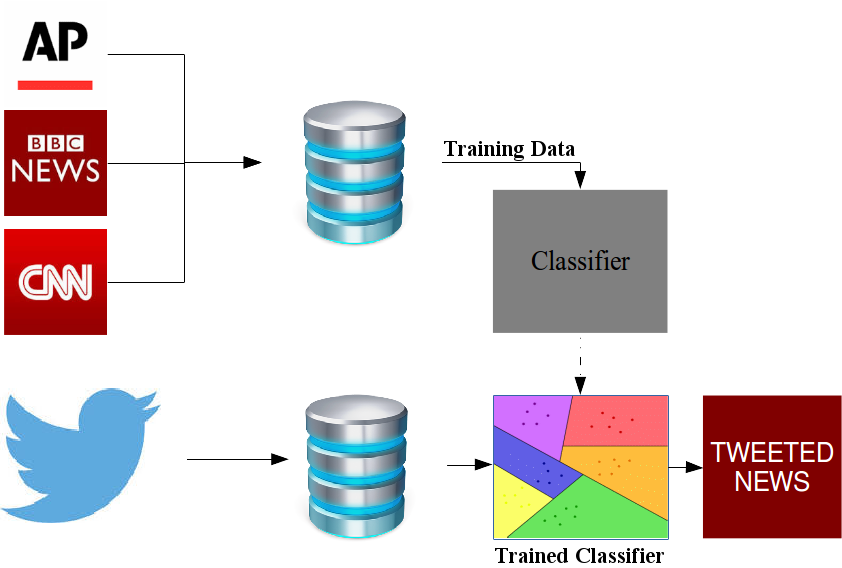
\includegraphics[width=0.8\textwidth]{images/bigpicture.png} 
  \caption{A big picture of the system}
  \label{fig:A big picture of the system}
\end{figure}

\section{Data collection}
We used different data sources and data storage systems. All the data collection tasks were performed using Python scripts.
\subsection{Data sources}
\subsubsection{Twitter data}
Twitter offer different ways of gathering data for different applications ~\cite{twitterdocumentation}. Unfortunately, giving access to the historic data is not one of them. In other words, our access to public data is limited to the most recent tweets. Hence, we decided to collect a large number of the most recent public tweets. 
Although Twitter Firehose ~\cite{twitterrestapi} offers access to all public tweets, it requires special permissions to access, which we could not acquire. Luckily, Twitter's \textit{Streaming API} ~\cite{twitterstreaming} can offer a large number of tweets: it streams a random subset (around one percent) of all the public tweets. This subset is large enough for our purpose. Moreover, the streaming API allows for a much faster collection of tweets in comparison to other APIs such as \textit{REST API}, and also does not have the rate limitations imposed by Twitter on its \textit{REST} APIs ~\cite{twitterdocumentation}. 


\subsubsection{News data}
We looked into different news agencies (CNN, BBC, Reuters, USA Today, The New York Times,...) and news aggregators (Feedzilla, Google News, Bing Search, ...) in order to collect the required data for training the classifier. Unfortunately, all such sources impose some rather strict limitations on the number of requests and results an agent can send and recieve. As an example, Feedzilla has a limitation of 100 results per request. Bing news is also a commercial product costs of which we cannot afford ~\cite{bingsearchapi}. Although we managed to collect a good amount of news using The New York Times ~\cite{thenytimes} and USA Today ~\cite{thenytimes} APIs, we gave them up for a better news source: Twitter accounts of the news agencies. 

All news agencies that we looked for have different twitter accounts for different news categories. For the first phase of the project, we chose to use the following news categories:

\begin{enumerate}
  \item Politics
  \item Sports
  \item Technology
\end{enumerate}

These categories are chosen due to the following facts:
\begin{itemize}
  \item There is not much overlap between these news categories (cf. business, technology, finance)
  \item The frequency of the news generated in these categories are significantly higher that other categories (couple of news items every hour)
\end{itemize}

We currently use the following Twitter accounts as our news sources: @CNNPolitics, @BBCPolitics, @ReutersPolitics, @BBCSport, @WorldSportCNN, @ReutersSports, @BBCTech, @CNNtech, @ReutersTech. Each account does not have more than some thousands of Tweets, and they do not Tweet more than a couple of news items per hour.

\subsection{Data storage}
To use the streaming API, the data collecting script needs to send an initial request and then keep listening for the stream of responses. Thus, we need to keep the script running on a server for a long period of time. Moreover, the API publishes more than 2000 tweets per second. This translates to around 20 gigabytes of tweets per day. This imposes a data storage problem, as our resources were rather limited at the first phase of the project. In order to address these issues, we managed to use one of the school's servers to run our script on. This server have around 200 GB of free space, which allows for almost 10 days of continous data collection. Moreover, we managed to use RAR ~\cite{wiki:RAR} compression to reduce the data size by a factor of 7. Nevertheless, since school servers are not the most reliable type of servers, we decided to take some precautions by setting up a home-based Raspberry Pi ~\cite{wiki:raspberrypi} server and connecting it to a 1-terabyte external hard disk drive. Using this setup, we are capable of collecting and storing around 350 days of twitter data using the \textit{Streaming API}.
\[\textit{Days of tweet collection}=\frac{\textit{Storage size}\times \textit{Compression ratio}} {\textit{Size of tweets per day}}\]
\[\frac{\textit{1000 GB} \times 7}{\textit{20 GB per day}}=\textit{350 days} \]

%\begin{figure}[H]
%  \centering
%  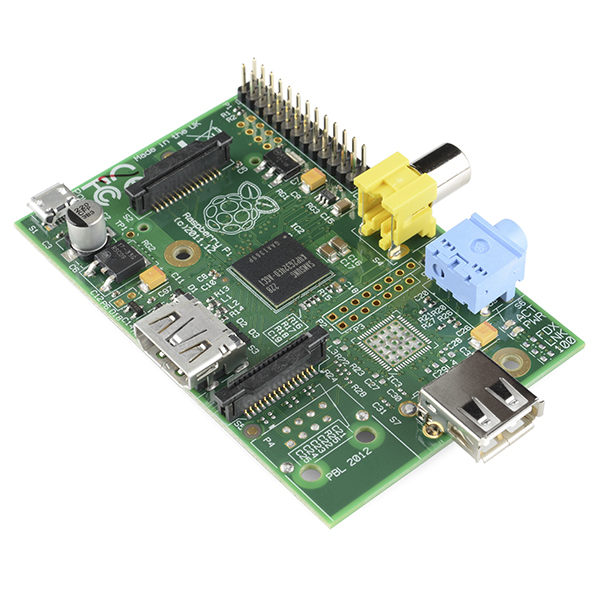
\includegraphics[width=0.5\textwidth]{images/rpi.jpg}
%  \caption{Raspberry Pi Setup / Image to be updated by Ali}
%  \label{fig:Raspberry Pi}
%\end{figure}

\section{Design of the system}

To select relevant tweets from the massive amount of twitter data, we will have to classify the tweets. By accurately assigning labels to tweets that describe their topics, we can find tweets that belong to our selected categories, i.e. "sports", "technology" or "politics". We used a Python machine learning package, Scikit ~\cite{scikit-learn}, which significantly simplified development of the classifier. A detailed diagram of the system is seen in Figure \ref{fig:System diagram}. 

\subsection{Classification}

\subsubsection{Feature extraction}
Traditionally, one would have to build a dictionary of the entire corpus that is being classified before being able to turn samples into feature vectors that can be used by a classifier. This would require at least one pass over the entire data set. We wish to prevent iterating over the entire data set multiple times, as this would be time consuming. To this end, feature hashing is used to turn texts into feature vectors without requiring a dictionary. The text is tokenized, stemmed and then hashed by a fast non-cryptographic hashing algorithm into a sparse feature vector. By choosing a sufficiently large feature space we minimize the risk of collisions. The generated feature vectors can then be used by a classifier.

\subsubsection{Choice of classifier}
The labeled training data (the news headlines) are processed by a stochastic gradient descent classifier. This type of classifier can converge on a solution without having to load the entire data set into memory. This makes it a great choice for this project, as we expect the data to grow beyond the memory bounds of a standard computer.

\begin{figure}[H]
  \centering
  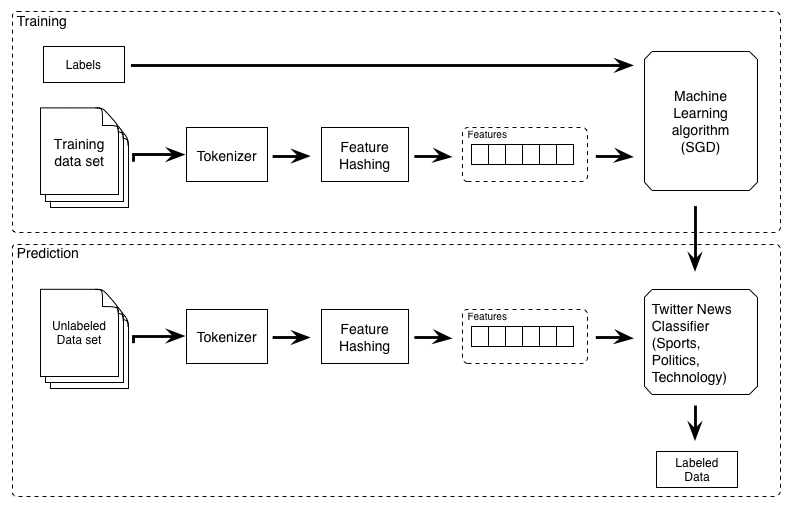
\includegraphics[width=\textwidth]{images/system.png}
  \caption{System diagram}
  \label{fig:System diagram}
\end{figure}

\section{Results}

To measure the quality of the classifier, we set aside a part of our training data and use that as test data. On this test data we measure several metrics, such as precision, recall and F1-score. These are presented in table \ref{tbl:classification-report} and they all display the same behavior: the classifiers are overly conservative in their predictions. This means that the predictions are trustworthy as evidence by a high precision metric. However, a lot of possibly relevant tweets are not given by these classifiers, which results in a low recall. In other words, we have a lot of false negatives. 

This behavior becomes even more clear in the confusion matrices displayed in figure \ref{fig:confusion-matrix}. The column-normalized confusion matrix shows that when a tweet gets classified into the categories "technology", "sports" and "politics", it is a very good prediction. In contrast, a lot of tweets that should actually be in "technology", "sports" or "politics" are classified as "other", as seen in the row-normalized confusion matrix.

\begin{table}
\begin{center}
\begin{tabular}{|r|r|r|r|r|} \hline
class  & precision   & recall & f1-score  & support \\ \hline
 technology    &   1.00 &     0.08  &    0.14   &   6195 \\
     sports   &    1.00   &   0.03   &   0.07   &   6365 \\
   politics   &    1.00  &    0.10   &   0.18   &   6376 \\
      other   &    0.79 &     1.00  &    0.88   &  65725 \\ \hline
avg / total  &     0.84   &   0.79  &    0.71   &  84661 \\ \hline
\end{tabular}
\end{center}
\caption{Classification performance over the three trained categories}
\label{tbl:classification-report}
\end{table}
 
\begin{figure}[H]
    \centering
    \begin{subfigure}[b]{0.48\textwidth}
        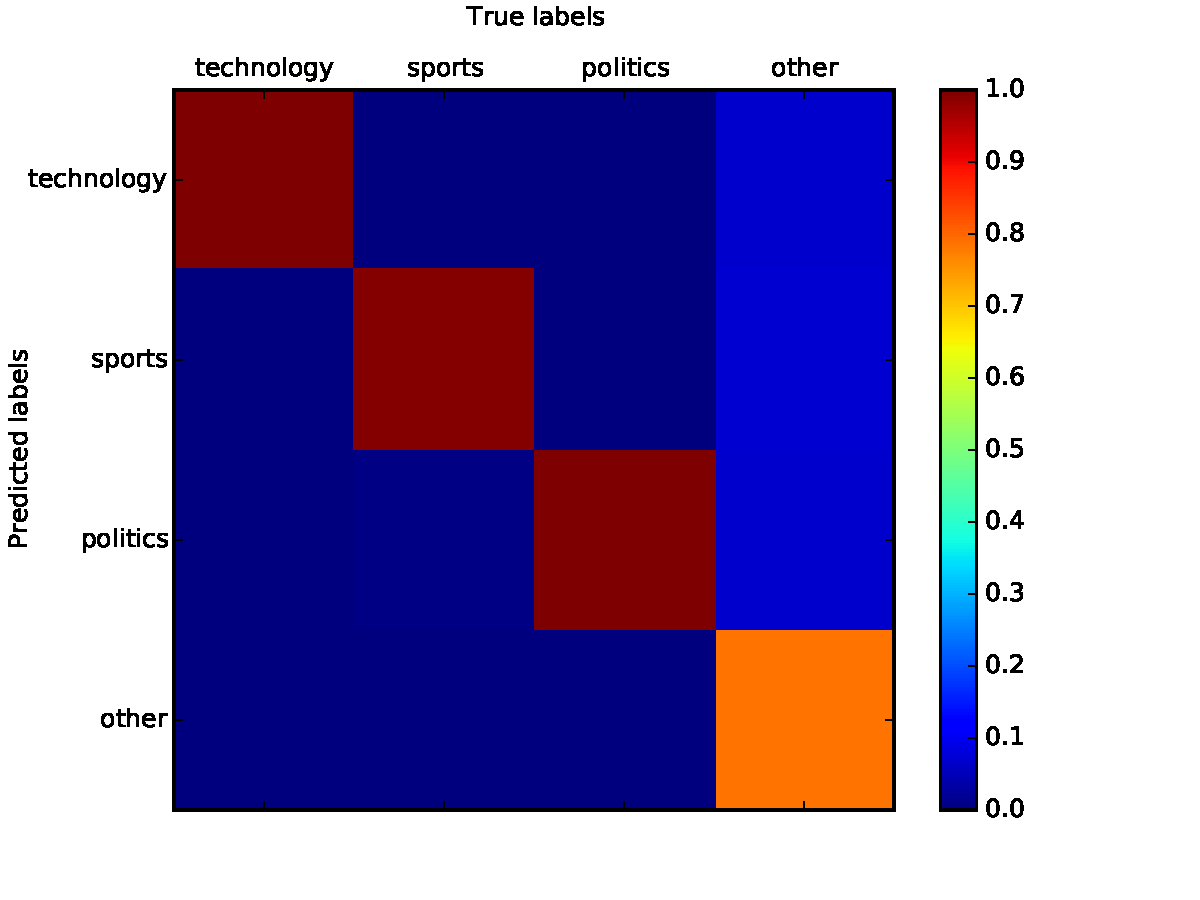
\includegraphics[width=\textwidth]{images/high-precision.pdf}
        \caption{Column-normalized confusion matrix}
        \label{fig:column-confusion-matrix}
    \end{subfigure}
    \begin{subfigure}[b]{0.48\textwidth}
        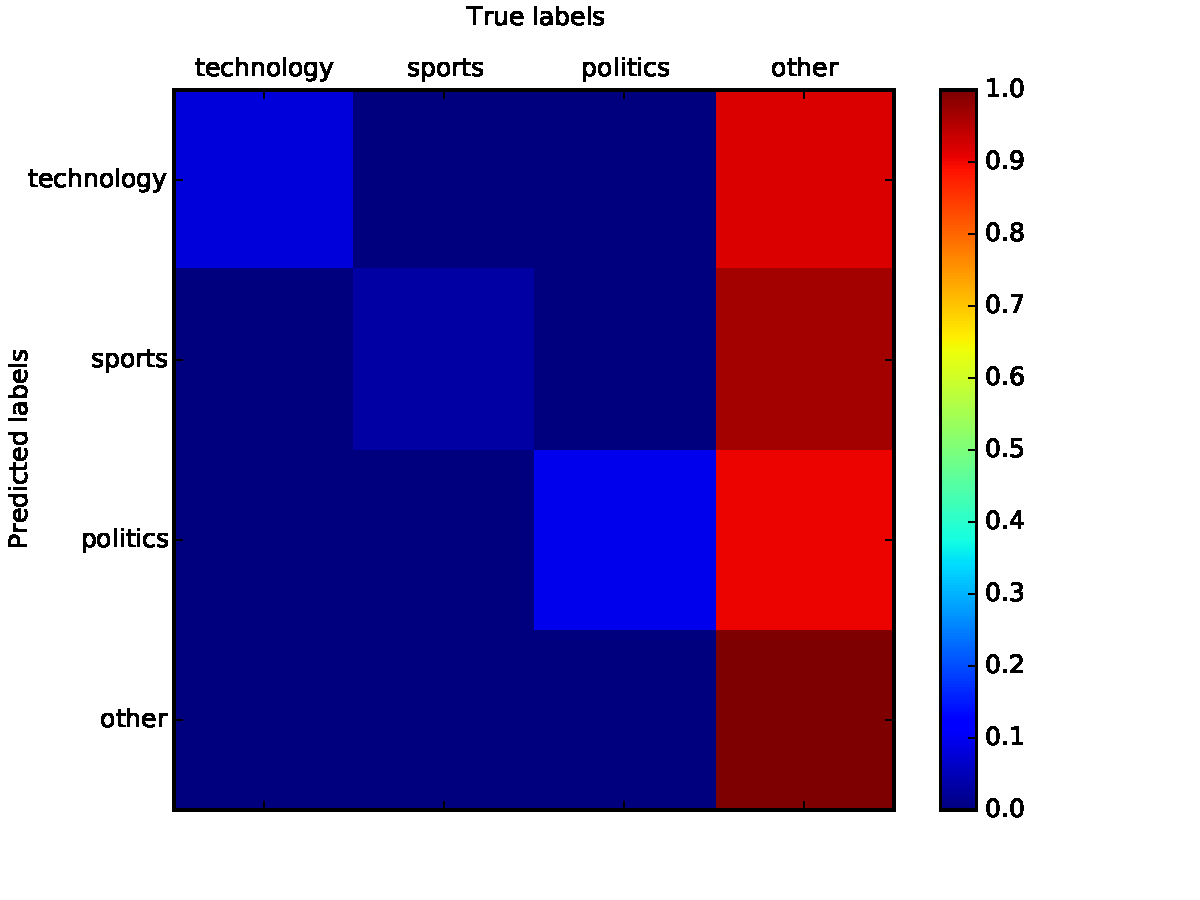
\includegraphics[width=\textwidth]{images/low-recall.pdf}
        \caption{Row-normalized confusion matrix}
        \label{fig:row-confusion-matrix}
    \end{subfigure}
    \caption{Confusion matrices of the three classifiers}
    \label{fig:confusion-matrix}
 \end{figure}
 
Due to the large amount of data, an overly conservative classifier is not necessarily a bad thing: even though we might be missing a lot of relevant tweets, we are still getting a large amount of useful predictions. 

\section{Future work}
The data size we worked on for the proof of concept phase is relatively small. For the next step of the project, we want to scale up the data size and add more features to enhance the news classifiers. 

We plan to run the massive data set on Spark and use MLlib, which is a Spark implementation of some common machine learning (ML) functionalities for massive data classification. Porting the training and prediction processes to Spark will be the challenge that we need to address in this phase. Another challenge will be optimizing the classifiers by giving different weights to the tweets, based on features like numbers of retweets, followers, and so on.

\bibliographystyle{plain}
\bibliography{report.bib}

\end{document}